\documentclass{article}
\usepackage{xltxtra}
\usepackage{xgreek}
\usepackage{amsmath}
\usepackage[ruled]{algorithm}
\usepackage{algorithmic}
\renewcommand{\O}{\mathcal{O}}

\usepackage{graphicx}
\graphicspath{ {./images/} }

\usepackage{amssymb}
\usepackage{amsthm}
%THEOREMS etc
\newtheorem{theorem}{Theorem}
\newtheorem{lemma}[theorem]{Lemma}

\setmainfont[Mapping=tex-text]{GFS Didot}

\begin{document}
\author{Νικόλαος Σμυρνιούδης (3170148)}
\title{Τρίτη προγραμματιστική εργασία - Μάθημα Αλγορίθμων}
\maketitle
\section{Άσκηση 3.3}
Οι δοκιμαστικές εκτελέσεις του αλγορίθμου έγιναν με την μέθοδο \\generateRandomGraph(int size) η οποία
δημιουργεί έναν γράφο μεγέθους size και προσθέτει κάθε ακμή με πιθανότητα 0.5 \\
\\
Ο αλγόριθμος εξαντλητικής αναζήτησης ελέγχει κάθε πιθανό υποσύνολο των κόμβων και συνεπώς τρέχει σε
χρόνο $\O(2^{|V|})$. Αυτό μπορεί να φανεί και απο τις παρακάτω πειραματικές εκτελέσεις αφού κάθε φορά που αυξάνεται
το πλήθος των κόμβων κατα ένα, ο απαιτούμενος χρόνος διπλασιάζεται. 
\begin{center}
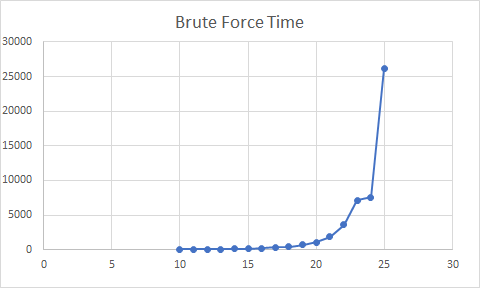
\includegraphics[width=10cm,height=10cm,keepaspectratio]{bruteforcetime}\\
\end{center}
Σε αντίθεση ο greedy αλγόριθμος χρειάζεται $\O(|V|^2)$ χρόνο (ο εξωτερικός βρόχος
τρέχει το πολύ $|V|$ φορές, removeVertex τρέχει το removeEdge το πολύ $|V|$ φορές, το findMax διατρέχει όλους τους κόμβους σε $|V|$ χρόνο)
και αυτό φαίνεται από τα πειράματα αφού για μικρές αλλαγές
δεν αλλάζει σημαντικά ο χρόνος εκτέλεσης.
\begin{center}
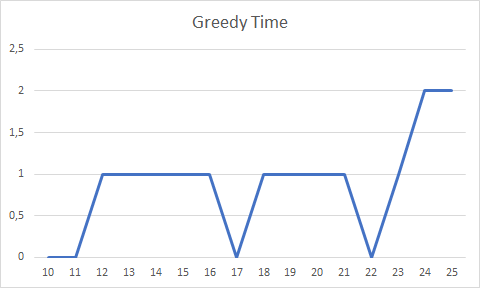
\includegraphics[width=10cm,height=10cm,keepaspectratio]{greedytime}\\
\end{center}
Τέλος, παρόλο που ο greedy αλγόριθμος βρίσκει VC με περισσότερους κόμβους απο το optimal VC του brute-force, αυτή η διαφορά δεν είναι μεγάλη και σίγουρα
δεν θα άξιζε να τρέξουμε τον brute-force αλγόριθμο μέχρι να σβήσει ο ήλιος για να βρούμε το optimal vertex cover για έναν γράφο με 100 κόμβους.  
\begin{center}
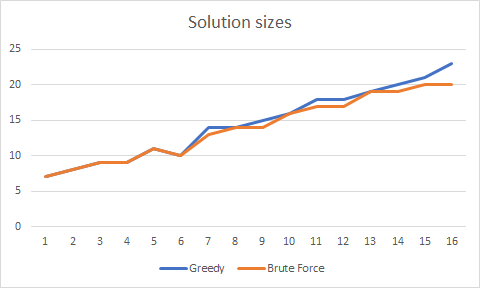
\includegraphics[width=10cm,height=10cm,keepaspectratio]{solutionsizes}\\
\end{center}
\section{Άσκηση 3.4}
Dominating Set:\\
\\
Δεδομένου γράφου $G(V,E)$ και ακεραίου $k$, υπάρχει $V' \subseteq V : \forall x \in V - V' : \exists y \in V' : \{x,y\} \in E$ με $|V'| = k$\\

Subset Cover:\\
\\
Δεδομένου συνόλου $S = \{x_1,..,x_n\}$ 
, υποσυνόλων του $S_1,...,S_m$ για τα οποία ισχύει $ S_{1} \cup ... \cup S_{m} = S $  
και ακεραίου $k$, υπάρχουν
$S_{x_1} ,..., S_{x_k}$ τέτοια ώστε
 $S_{x_1} \cup ... \cup S_{x_k} = S $ \\

Ακολουθεί ένα λήμμα που θα είναι χρήσιμο στην αναγωγή
\begin{lemma}
\label{DSk_subset_Dsk+1}
	Έστω $G(V,E)$ γράφος και $V'$ dominating-set. Άν προσθέσουμε οποιονδήποτε κόμβο απο το $V-V'$ στο $V'$,το τελικό
	$V'$ παραμένει dominating-set.
\end{lemma}
\textit{Απόδειξη:}\\
	Έστω $v \in V - V'$. Λόγω του $V'$ , $\forall x \in V - V' : \exists y \in V' : \{x,y\} \in E$ .
	Και επειδή $V - (V' \cup \{v\}) \subseteq V-V'$ και $V' \subseteq V' \cup\{v\}$ τότε θα ισχύει και:
	$$
		\forall x \in V-(V' \cup \{v\}) : \exists y \in  V' \cup \{v\} : \{x,y\} \in E .
	$$
	Άρα τελικά το $V' \cup \{v\}$ είναι dominating-set.
\begin{theorem}
Το πρόβλημα Dominating Set είναι NP-complete\\
\end{theorem}
	\begin{proof}
	\begin{itemize}
		\item Dominating Set $\in NP$\\
	\end{itemize}	
		Έστω $V'$ το Dominating Set με μέγεθος k. Ο αλγόριθμος 1 ελέγχει σε πολυωνυμικό χρόνο
		αν όντως το $V'$ είναι Dominating Set.
		
		Ο εξωτερικός βρόχος τρέχει το πολύ $V$ φορες, εσωτερικός σε $Ε$ ενώ το αν μεσα στον
		εσωτερικό βρόχο χρειάζεται να διατρέξει το σύνολο $V'$ σε $k$ βήματα. Συνολικά, ο χρόνος για να ελεγχθεί μια λύση του Dominating Set
		είναι $\O(V*E*k)$.
	\begin{itemize}		
		\item SUBSET-COVER $\leq _p$ DOMINATING-SET:\\
	\end{itemize}		
		Η γενική ιδέα της αναγωγής είναι να παράξουμε εναν γράφο όπου κάθε στοιχείο τους συνόλου S είναι ενας κόμβος
		στο σύνολο X, και επίσης κάθε δεδομένο υποσύνολο του S είναι ένας κόμβος στο σύνολο H. Μετά προστίθενται ακμές στον
		γράφο ετσι ώστε αν υπάρχει DOMINATING-SET k μεγέθους αυτό να είναι ένα υποσύνολο του H μεγέθους k δηλαδή μια λύση στο
		πρόβλημα του SUBSET-COVER.\\
		  
		Οι κόμβοι του παραχτέου γράφου θα έχουν ένα πεδίο .d το οποίο θα είναι ενα σύνολο.\\
		Έστω $X = \{x_i| x_i \in S\}$. Θέτουμε για κάθε στοιχείο του $X$ , $x_i.d = \emptyset$.\\
		Θεωρούμε το σύνολο $Η = \{h_i | i = 1,..,m\}$
		Θέτουμε  $h_i.d = S_i , i = 1,..,m$. Οι κόμβοι του γράφου θα έιναι το σύνολο $V = T \cup X$. Όσο για
		τις ακμές θεωρούμε τα σύνολα $E_1 = \{\{u,v\} | u,v \in  T \}$ , $E_2 = \{\{x_i,v\} | x_i \in S , v \in T \text{ και } x_i \in v  \}$
		και θέτουμε ώς σύνολο ακμών το $E = E_1 \cup E_2$\\
		\\
		Έτσι έχουμε δημιουργήσει μια συνάρτηση  $f(S,S_1,...,S_m,k) = (G(V,E) , k)$ απο στιγμιότυπα του SUBSET-COVER σε στιγμιότυπα του DOMINATING
		SET.
		\begin{lemma}
			Το στιγμιότυπο $(S,S_1,...,S_m,k)$ του SUBSET-COVER είναι ναι ανν το $(G(V,E) , k)$ στιγμιότυπο του DOMINATING-SET που παράγεται είναι ΝΑΙ
		\end{lemma}
		\textit{Απόδειξη:}\\
		\\
		\textit{$\Longrightarrow$} Έστω πώς υπάρχουν $k$ υποσύνολα απο τα δεδομένα τ.ω. $ S_{p_1} \cup ... \cup S_{p_k} = S $. Τότε για το υποσύνολο κόμβων
					 του γράφου που παράγεται μέσω της $f$, το $V'= \{h_{p_i} | i=1,..,k \}$, ισχύει πώς για κάθε κόμβο του γράφου που δεν βρίσκεται
					 στο $V'$, αυτός έχει τουλάχιστον έναν γείτονα στο $V'$. Οι κόμβοι που βρίσκονται στο σύνολο $H-V'$, έχουν γείτονες όλους
					 τους κόμβους στο σύνολο $V'$. Οι κόμβοι του συνόλου $X$ έχουν όλοι τουλάχιστον έναν γείτονα στο σύνολο $V'$ 
					 (επειδή $h_{p_1}.d \cup ... \cup h_{p_k}.d = S $).   
		       		 Προφανώς, το μέγεθος του $V'$ είναι $k$ και συνεπώς είναι DOMINATING-SET $k$ μεγέθους.\\
		       		 \\
		\textit{$\Longleftarrow$} 
			Έστω το dominating-set μεγέθους $k$ $V' = X' \cup H'$ με $H' \subseteq H , X' \subseteq X$. Για κάθε στοιχείο του $X'$ θα υπάρχει τουλάχιστον ενα
			στοιχείο του $H$ το οποίο να είναι γειτονικό. Θεωρούμε το σύνολο $H''$ το οποίο περιέχει έναν αυθαίρετο γείτονα κάθε στοιχείου στο $X'$. Επειδή
			$H'' \subseteq X'$ θα ισχύει: $|H' \cup H''| \leq |H' \cup X'| \leq k$.
			\\
			Μένει να αποδειχτεί πως $H' \cup H''$ είναι dominating-set.
			Πράγματι για κάθε $v \in H - (H' \cup H'')$ ο $v$ θα έχει έναν γείτονα στο $H' \cup H''$ (ολοι οι κόμβοι στο $H$ συνδέονται με όλους στο $H$).
			Eπειδή το $X'\cup H'$ είναι dominating-set και επειδή δεν υπαρχουν δυο κόμβοι στο $X$ που να συνδέονται μεταξύ τους, για τούς $v \in X - X'$
			ισχύει πως θα έχουν όλοι κάποιον γείτονα στο $H'$ αρα και στο $ H' \cup H''$. Τέλος, οι κόμβοι του $X$ που βρίσκοταν στο παλιό DS, δηλαδή οι 
			$v \in X'$ θα έχουν όλοι κάποιον γείτονα στο $H'$ λόγω του πως ορίστικε το $H'$. Καταλήγουμε τελικά πως για κάθε $v \in V -(H' \cup H'')$ ο $v$
			έχει κάποιον γείτονα στο $H' \cup H''$. Αν το μέγεθος του $H' \cup H''$ είναι μικρότερο απο $k$ μπορούμε να προσθέσουμε ,σύμφωνα με το λήμμα 1,
			οποιονδήποτε αριθμό κόμβων απο το $H-(H' \cup H'')$ στο $(H' \cup H'')$ μέχρι αυτό να γίνει DS k στοιχείων.\\
			Επειδή όλα τα στοιχεία του $X$ έχουν γείτονα στο  $(H' \cup H'')$ αυτό σημαίνει πως $$\bigcup_{h_i \in (H' \cup H'')}h_i.d = S$$ άρα και υπάρχει
			σύνολο υποσυνόλων k στοιχείων που να κάλύπτει το $S$.
 			
	Τέλος, επειδή το SET-COVER είναι NP-complete , τότε και το DOMINATING-SET θα έιναι NP-complete.
	\end{proof}
\begin{algorithm}
		\caption{checkDS($G(V,E),V')$)}
		\label{s}
		\begin{algorithmic}[1]
			\FOR{ every $x \in V - V'$}
				\STATE found = false
				\FOR {every $\{u,v\} \in G.E $}
					\IF{$(u = x \text{ AND } v \in V') \text{ OR } (v == x \text{ AND } u \in V')$}
						\STATE found = true;
					\ENDIF
				\ENDFOR
				\IF{found == false}
					\RETURN{false}
				\ENDIF
			\ENDFOR 
			\RETURN{true}
		\end{algorithmic}
		\end{algorithm}
\end{document} 

